\documentclass[12pt, a4paper]{article}
\usepackage{indentfirst}
\usepackage{graphicx}
\usepackage{url}
\def\UrlBreaks{\do\/\do-}
\usepackage{cite}
\usepackage{float}
\usepackage[font=footnotesize,labelfont=bf]{caption}
\graphicspath{{images/}}
\title{GDPR: Is non-compliance profitable for Meta Platforms, Inc.?}
\author{Stoyan L. Kostadinov}
\date{June 2023}
\begin{document}
\maketitle

\begin{center}
    
\includegraphics[width=0.3\textwidth]{fontys-logo}
\end{center}

\begin{abstract}
    % TODO
\end{abstract}

\subsection*{Keywords}

GDPR, Facebook, Meta, profit, non-compliance, privacy, financial impact

\section*{Introduction}

In the recent years, the increasing usage of the Internet has lead to a rapid
expansion of data collection and processing\cite{khan2014big}. As concerns
regarding data privacy and protection grew, the European Union (EU) implemented
the General Data Protection Regulation (GDPR) in May
2018\cite{greengard2018weighing, historyGdpr}.

GDPR aimed to safeguard the privacy rights of individuals within the EU by
regulating the collection, storage, and transfer of personal
data\cite{historyGdpr}. Notably, data should be collected for specified,
explicit and legitimate purposes\cite{europeanParliamentGdprArticle5} and data
can be transferred outside the EU if general data processing principles are in
place \cite{europeanParliamentGdprArticle44}. Compliance with GDPR has become a
critical issue for big-tech companies, which often handle massive amounts of
user data.

One of those companies is \textit{Meta Platforms, Inc.} (formerly
\textit{Facebook, Inc.}), which has been fined numerous times for GDPR
violations\cite{mrevzar2023analysis}. This has raised questions about the impact
of GDPR on \textit{Meta's} performance.

The goal of this paper is to investigate the financial impact of GDPR
non-compliance on \textit{Meta Platforms, Inc.} and to determine whether it is
profitable for the company to continue violating the regulations.

\section*{Method}

All numerical data about \textit{Meta Platforms, Inc.} has been gathered from
the official \textit{Meta Investor Relations} website\cite{fbMetaFinancials} -
\textbf{Balance Sheets}, \textbf{Income Statements} and \textbf{Form 10-Q}.
Stock performance data has been gathered from the official \textit{Yahoo!
Finance} website\cite{stockPrice}.

GDPR fines imposed on \textit{Meta Platforms, Inc.} have been gathered from the
\textit{GDPR Enforcement Tracker}
website\cite{enforcementtrackerGDPREnforcement} and filtered to include fines
imposed on their family of applications (\textbf{\textit{Facebook}},
\textbf{\textit{WhatsApp}}, \textbf{\textit{Instagram}}) and
\textbf{\textit{Meta Platforms, Inc.}} itself.

\subsection*{Inclusion criteria}

\begin{itemize}
    \item Articles published in English
    \item Articles published after 2010
    \item Data about GDPR fines
    \item Data about \textit{Meta Platforms, Inc.} financials
    \item Data between 2018 and 2023
\end{itemize}

\subsection*{Exclusion criteria}

\begin{itemize}
    \item Articles published in languages other than English
    \item Articles published before 2010
    \item Data that is not about GDPR fines
    \item Data that is not about \textit{Meta Platforms, Inc.} financials
    \item Data before 2018
\end{itemize}

\subsection*{Ethical considerations}

This study is approved by \textit{Fontys University of Applied Sciences,
Eindhoven, The Netherlands}. All data is collected from publicly available
sources and no personal data is collected. The author is not affiliated with
\textit{Meta Platforms, Inc.} or any other company mentioned in this study.

\section*{Results}

\subsection*{GDPR Fines}

\begin{figure}[H]
    \centering
    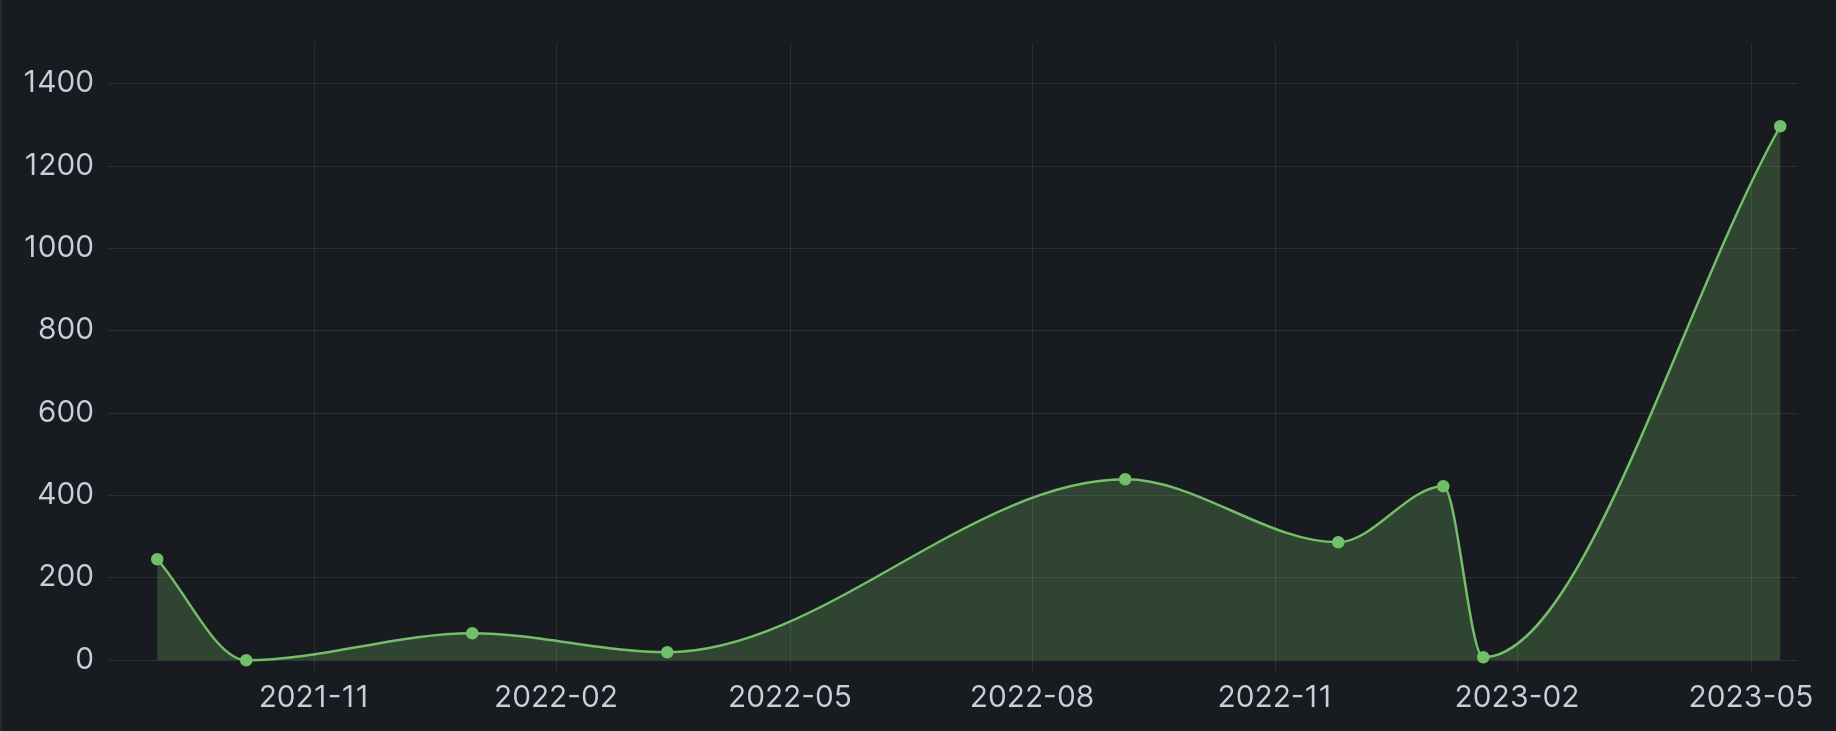
\includegraphics[width=1.00\textwidth]{monetarial-amount-of-gdpr-fines}
    \caption{Monetarial amount of fines issued to Meta Platforms, Inc.(in
    millions of
    \$)\cite{gdprFine1,gdprFine2,gdprFine3,gdprFine4,gdprFine5,gdprFine6,gdprFine7,gdprFine8,gdprFine9}}
    \label{fig:amount-of-gdpr-fines}
\end{figure}

% \begin{figure}[H]
%     \centering
%     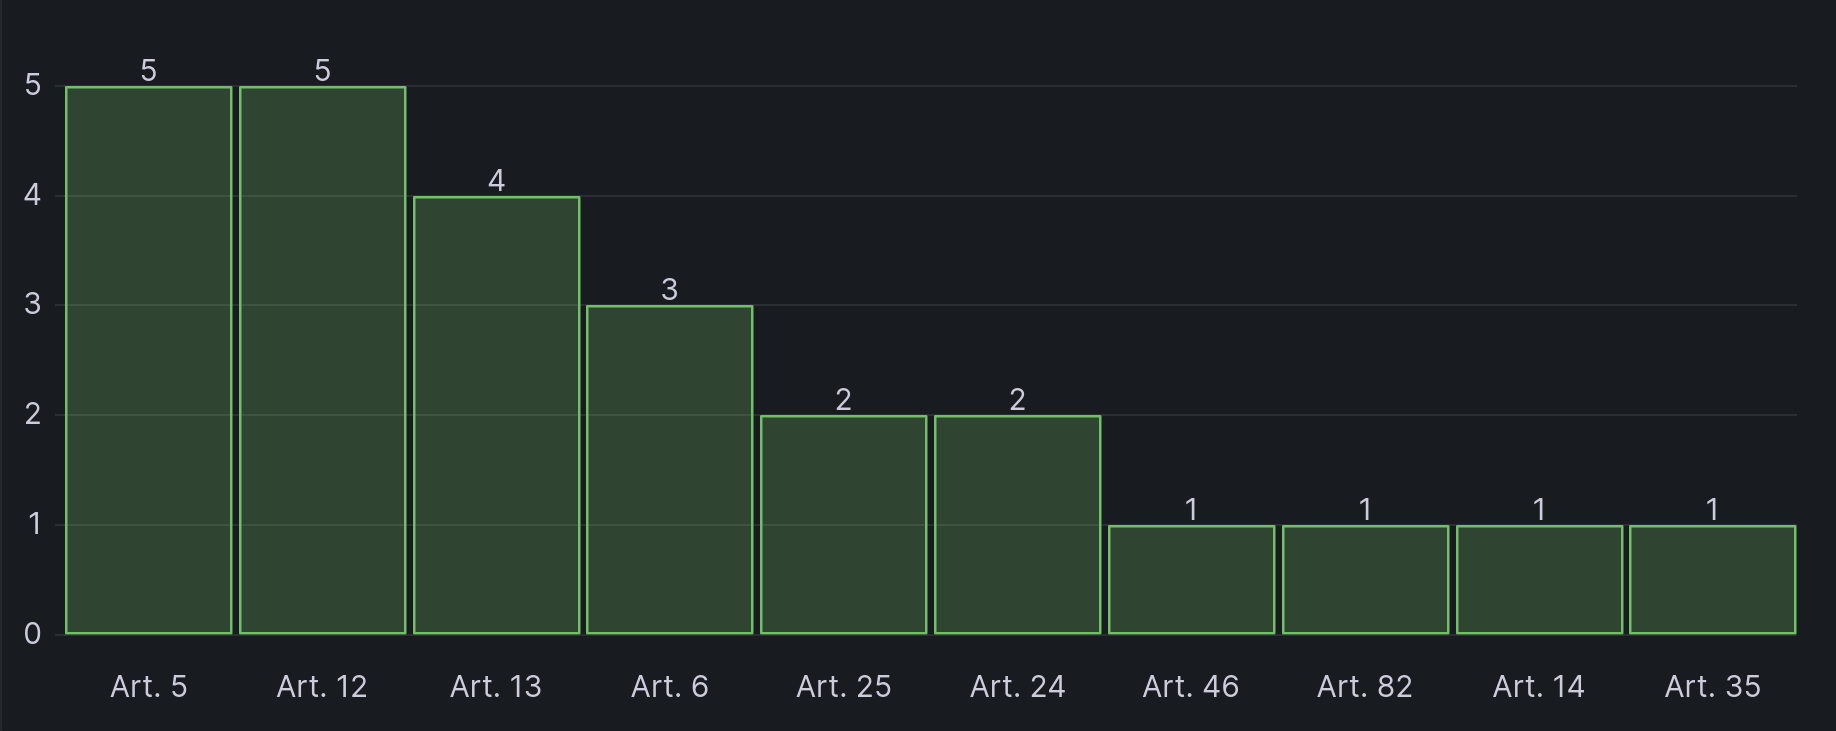
\includegraphics[width=1.00\textwidth]{violations-by-article}
%     \caption{Number of violations by GDPR
%     article\cite{gdprFine1,gdprFine2,gdprFine3,gdprFine4,gdprFine5,gdprFine6,gdprFine7,gdprFine8,gdprFine9}}
%     \label{fig:violations-by-article}
% \end{figure}

\subsection*{Financials}

\begin{figure}[H]
    \centering
    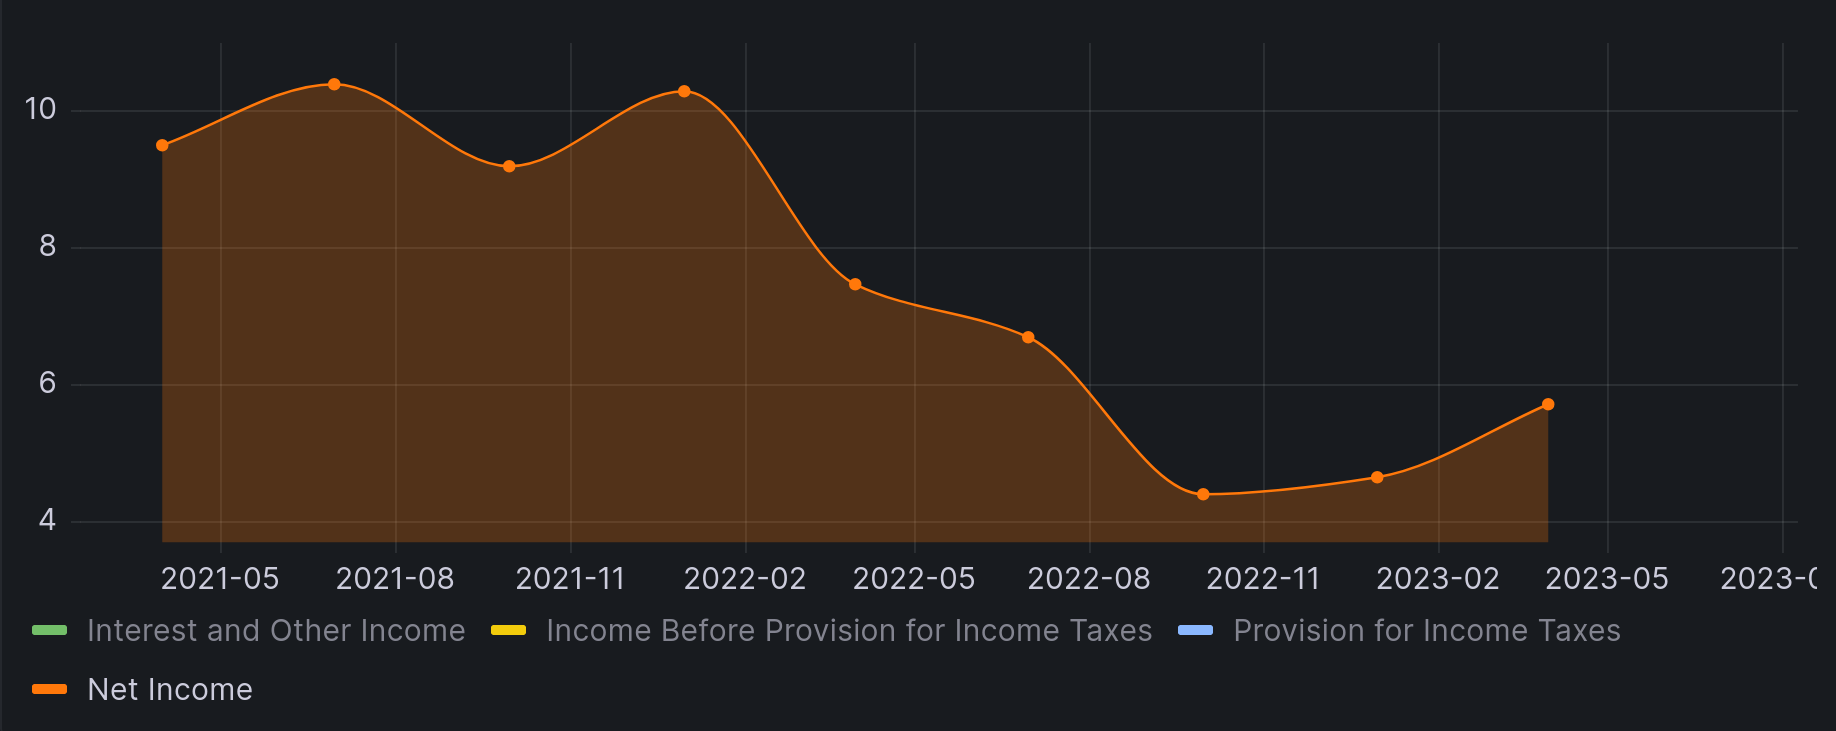
\includegraphics[width=1.00\textwidth]{net-income}
    \caption{Net Income of Meta Platforms, Inc.(in billions of
    \$)\cite{2023q1,2020q4,2020q3,2020q2,2020q1,2019q4,2019q3,2019q2,2019q1,2018q4,2018q3,2018q2}}
    \label{fig:net-income}
\end{figure}

\begin{figure}[H]
    \centering
    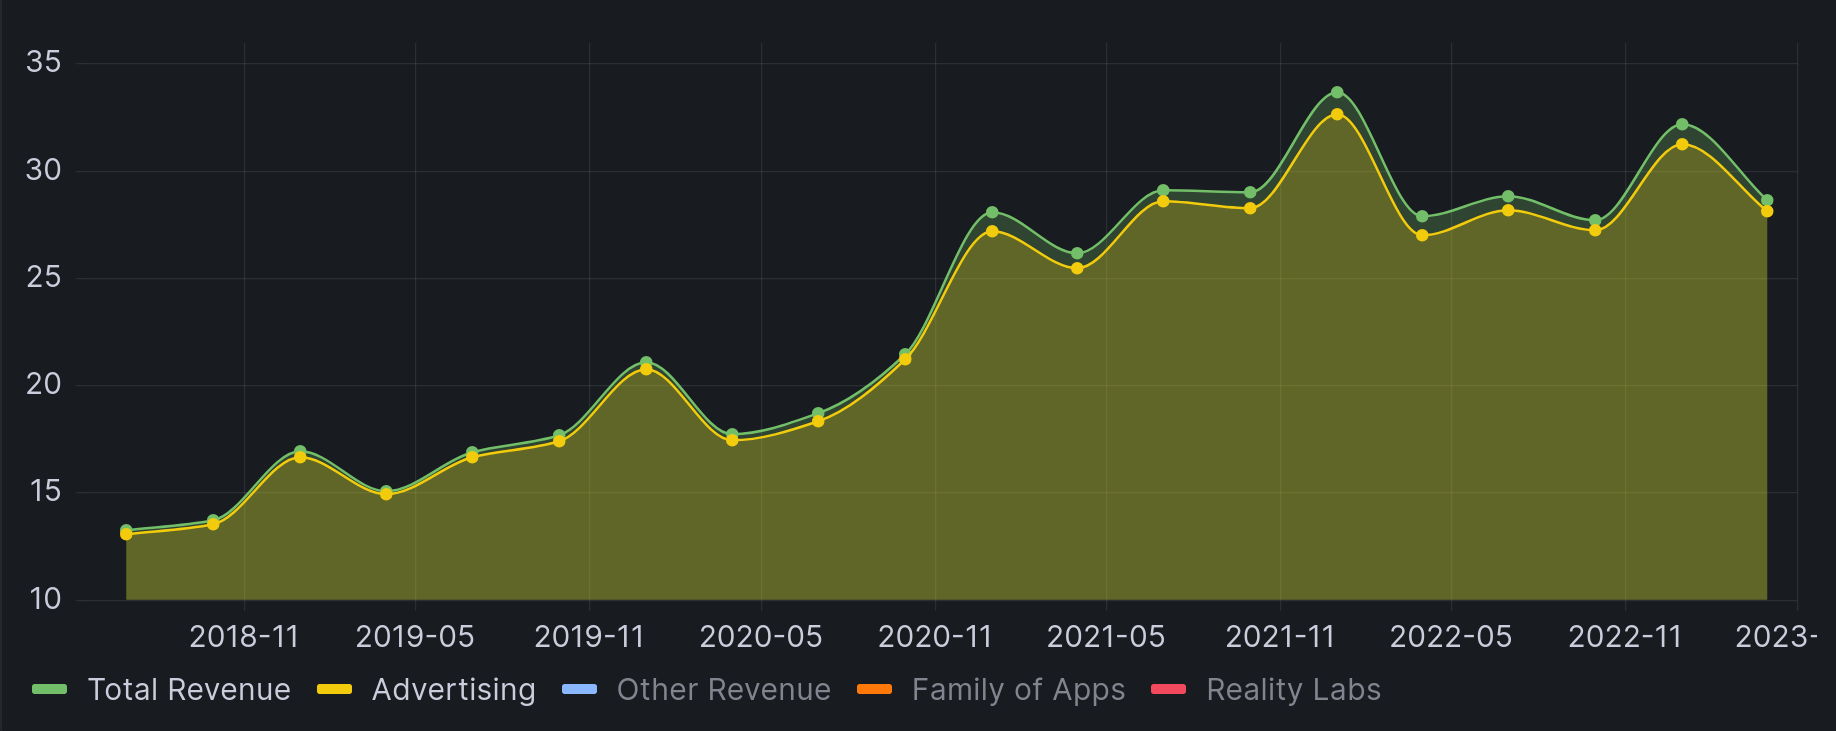
\includegraphics[width=1.00\textwidth]{revenue}
    \caption{Revenue of Meta Platforms, Inc.(in billions of
    \$)\cite{2023q1,2020q4,2020q3,2020q2,2020q1,2019q4,2019q3,2019q2,2019q1,2018q4,2018q3,2018q2}}
    \label{fig:revenue}
\end{figure}

\subsection*{Investor Confidence and Stock Performance}

\begin{figure}[H]
    \centering
    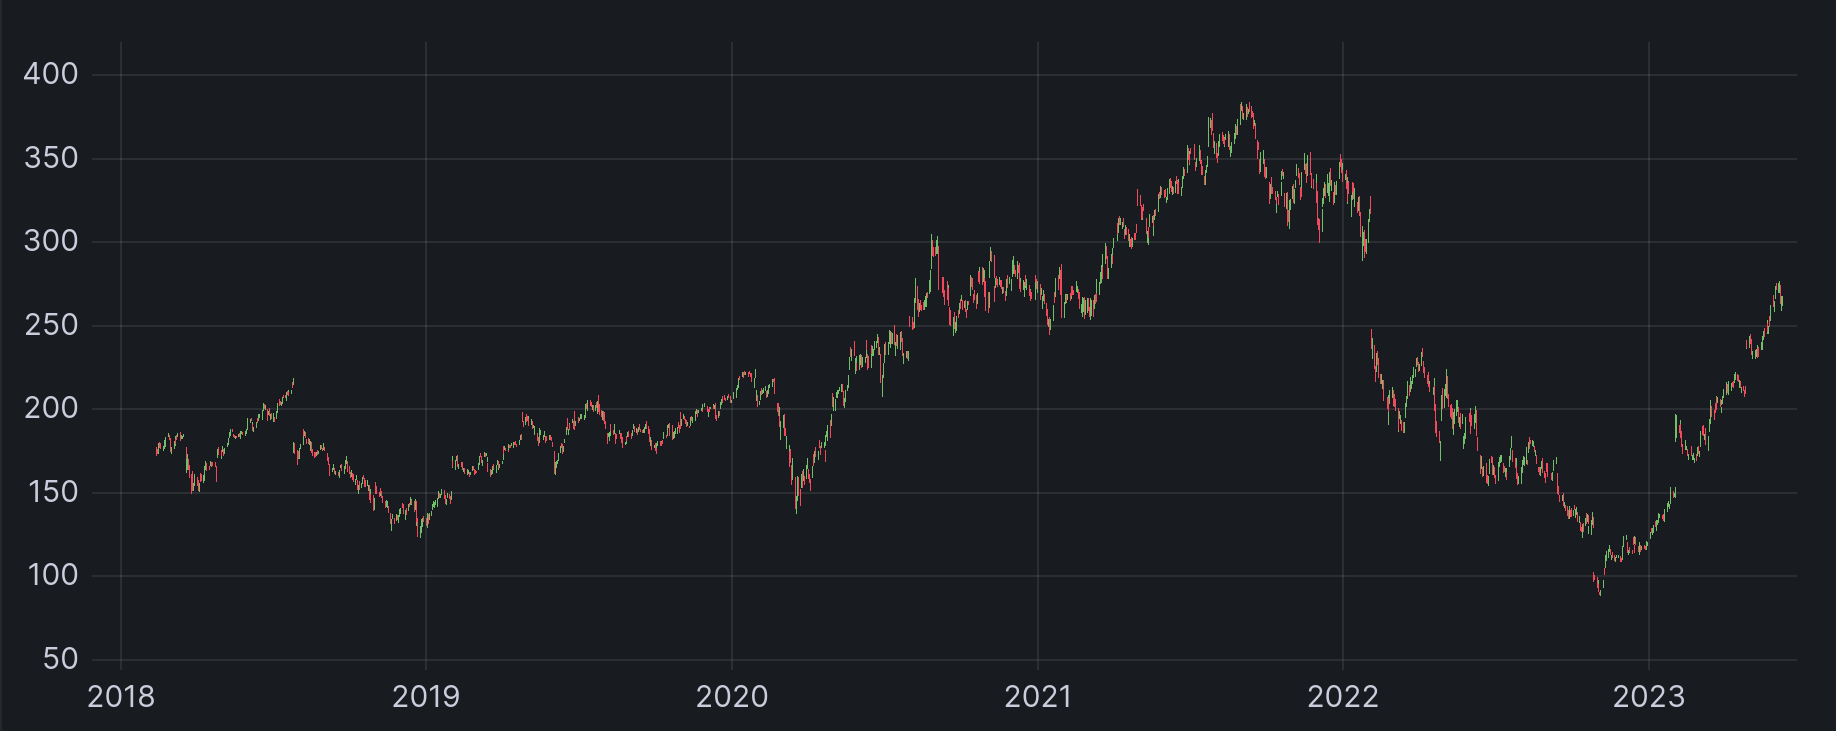
\includegraphics[width=1.00\textwidth]{stock-price}
    \caption{Stock Price Performance of Meta Platforms, Inc. (META) (in
    \$)\cite{stockPrice}}
    \label{fig:stock-price}
\end{figure}

\begin{figure}[H]
    \centering
    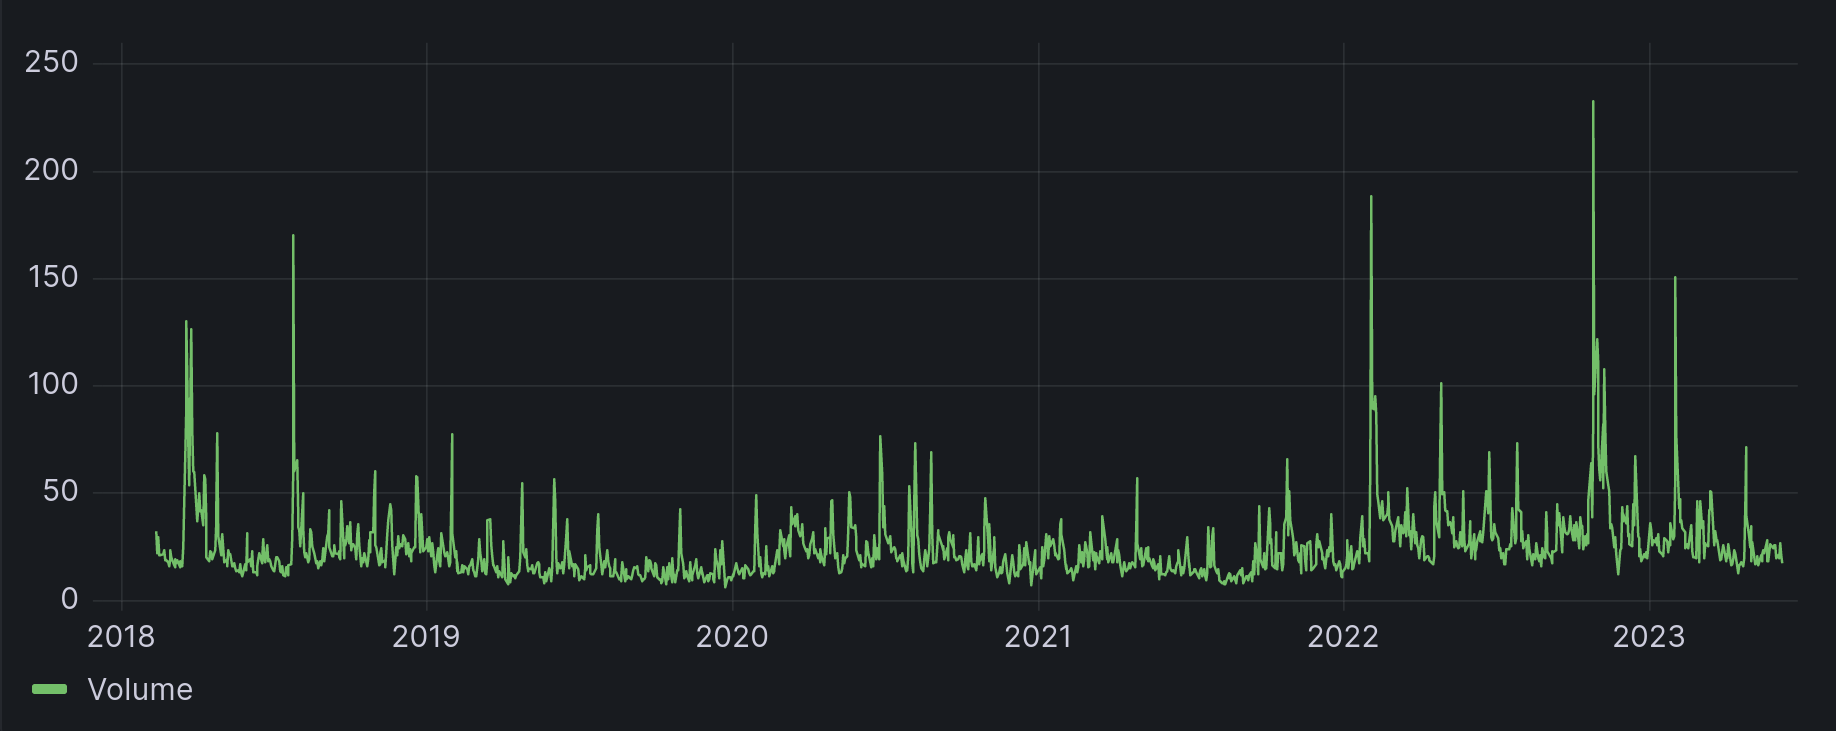
\includegraphics[width=1.00\textwidth]{volume}
    \caption{Volume of Meta Platforms, Inc. (META) (in millions of
    shares)\cite{stockPrice}}
    \label{fig:volume}
\end{figure}

\subsection*{Advertising}

\begin{figure}[H]
    \centering
    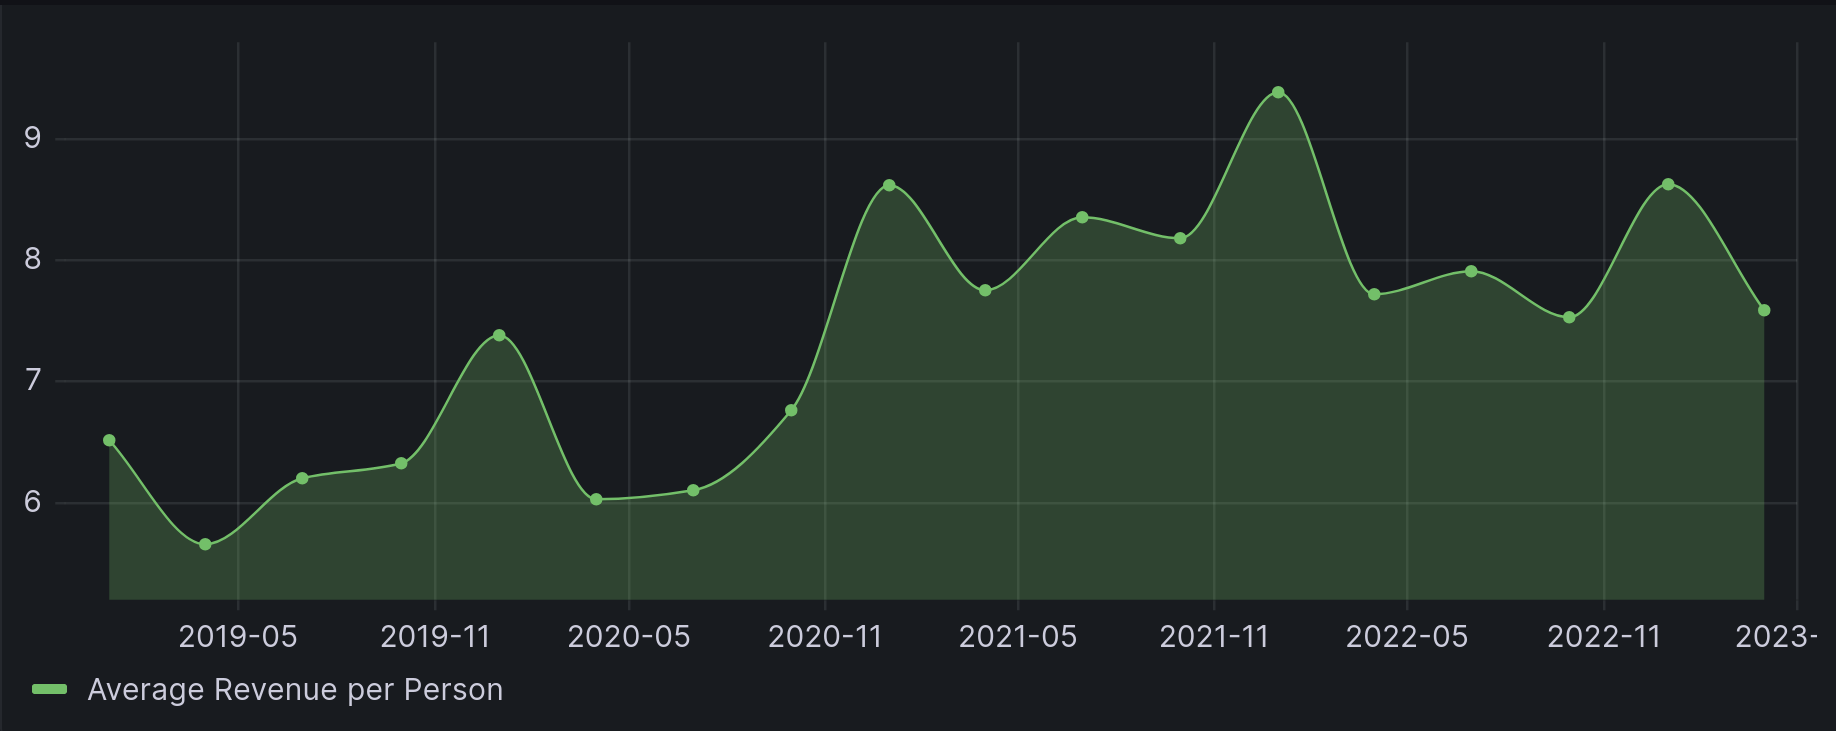
\includegraphics[width=1.00\textwidth]{family-revenue-per-person}
    \caption{Family Revenue per Person (FRP) of Meta Platforms,
    Inc.\cite{2023q1,2021q2Slides,2019q4Slides}}
    \label{fig:family-revenue-per-person}
\end{figure}

\begin{figure}[H]
    \centering
    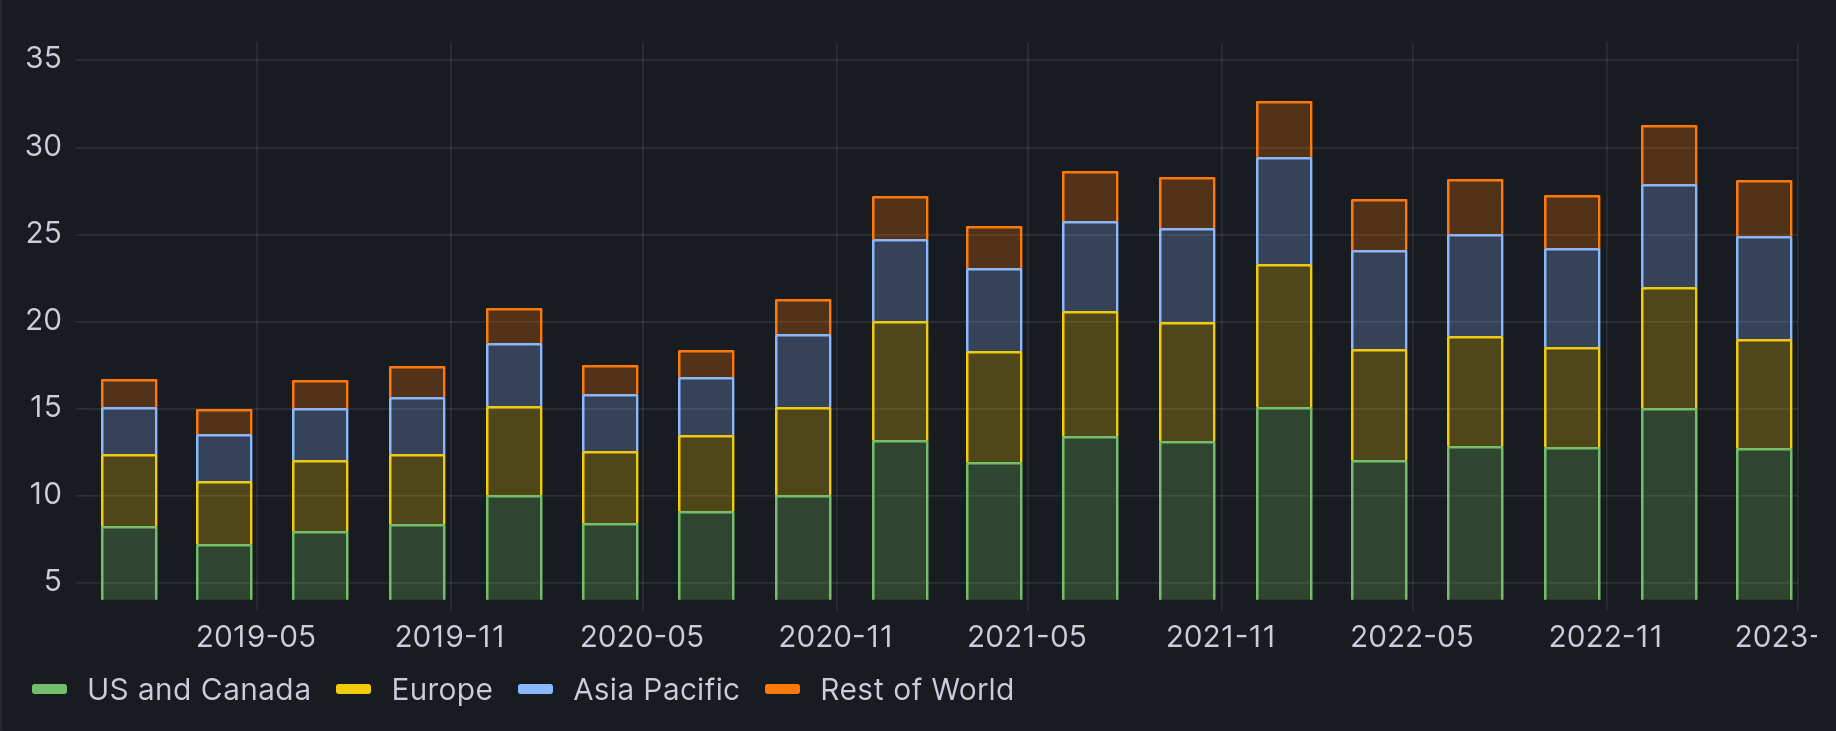
\includegraphics[width=1.00\textwidth]{advertising-revenue-by-user-geography}
    \caption{Advertising Revenue by User Geography of Meta Platforms, Inc.(in
    billions of \$)\cite{2023q1,2021q2Slides,2019q4Slides}}
    \label{fig:advertising-revenue-by-user-geography}
\end{figure}

\subsection*{User Base and User Engagement}

\begin{figure}[H]
    \centering
    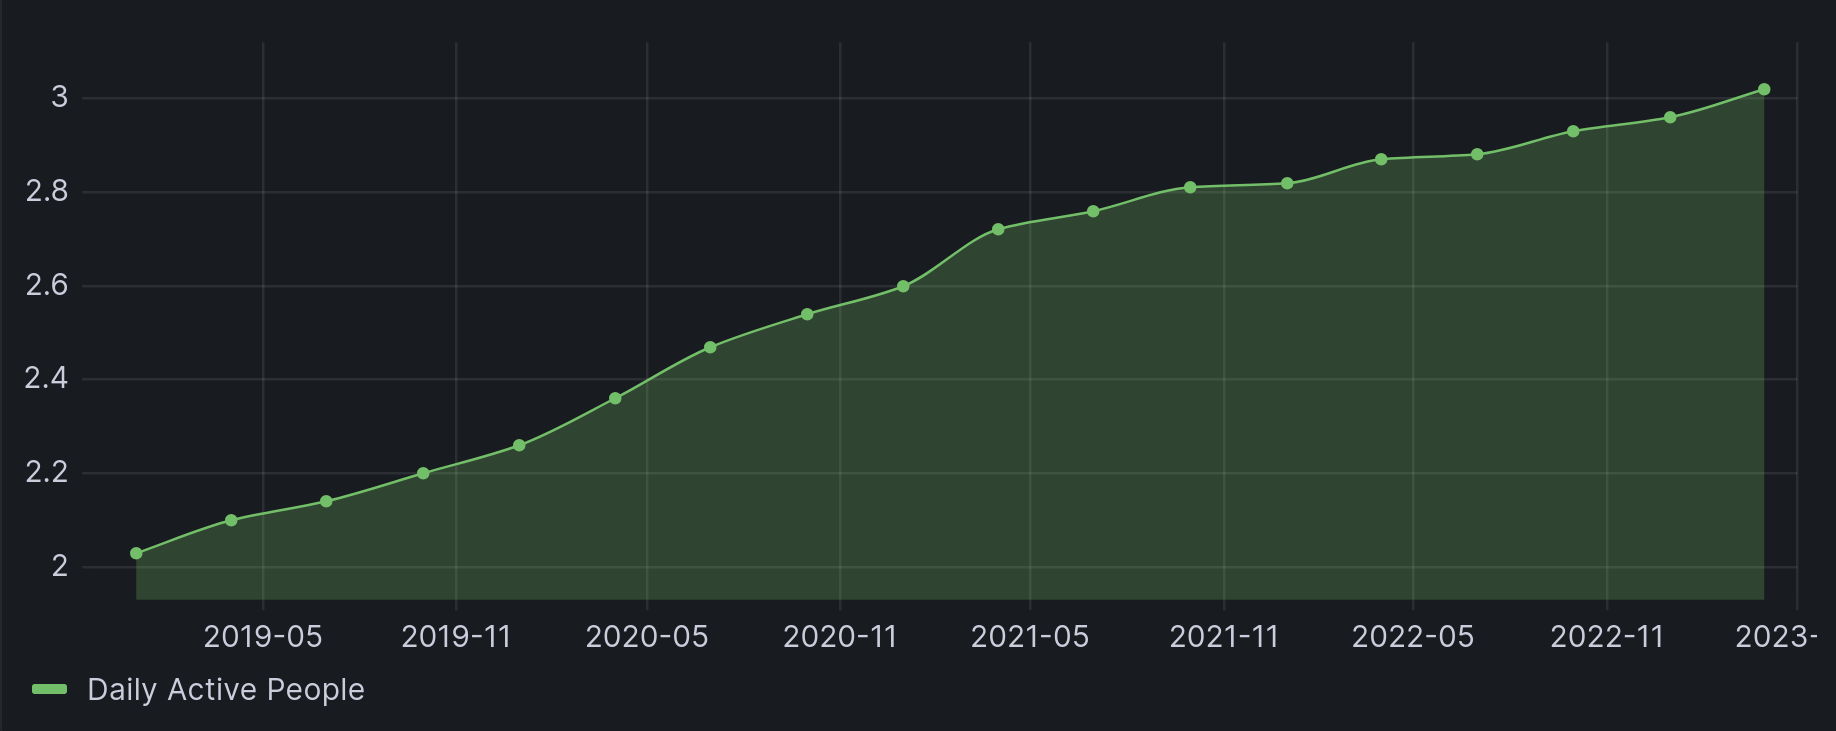
\includegraphics[width=1.00\textwidth]{family-dap}
    \caption{Family Daily Active People (FDAP) of Meta Platforms, Inc.(in
    billions)\cite{2023q1,2021q2Slides,2019q4Slides}}
    \label{fig:family-dap}
\end{figure}

\begin{figure}[H]
    \centering
    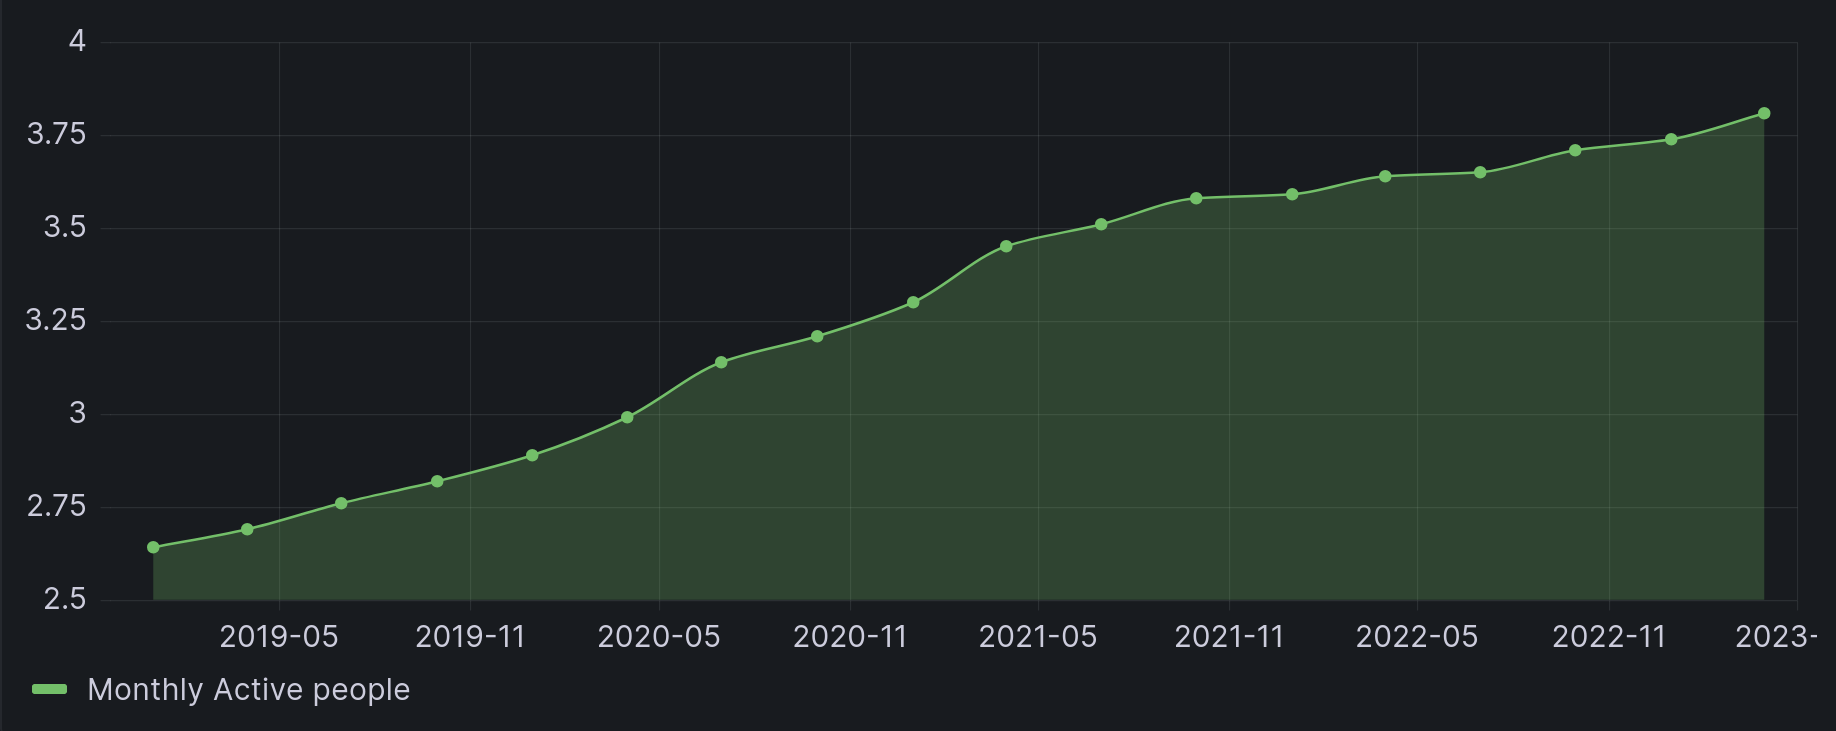
\includegraphics[width=1.00\textwidth]{family-map}
    \caption{Family Monthly Active People (FMAP) of Meta Platforms, Inc.(in
    billions)\cite{2023q1,2021q2Slides,2019q4Slides}}
    \label{fig:family-map}
\end{figure}

\begin{figure}[H]
    \centering
    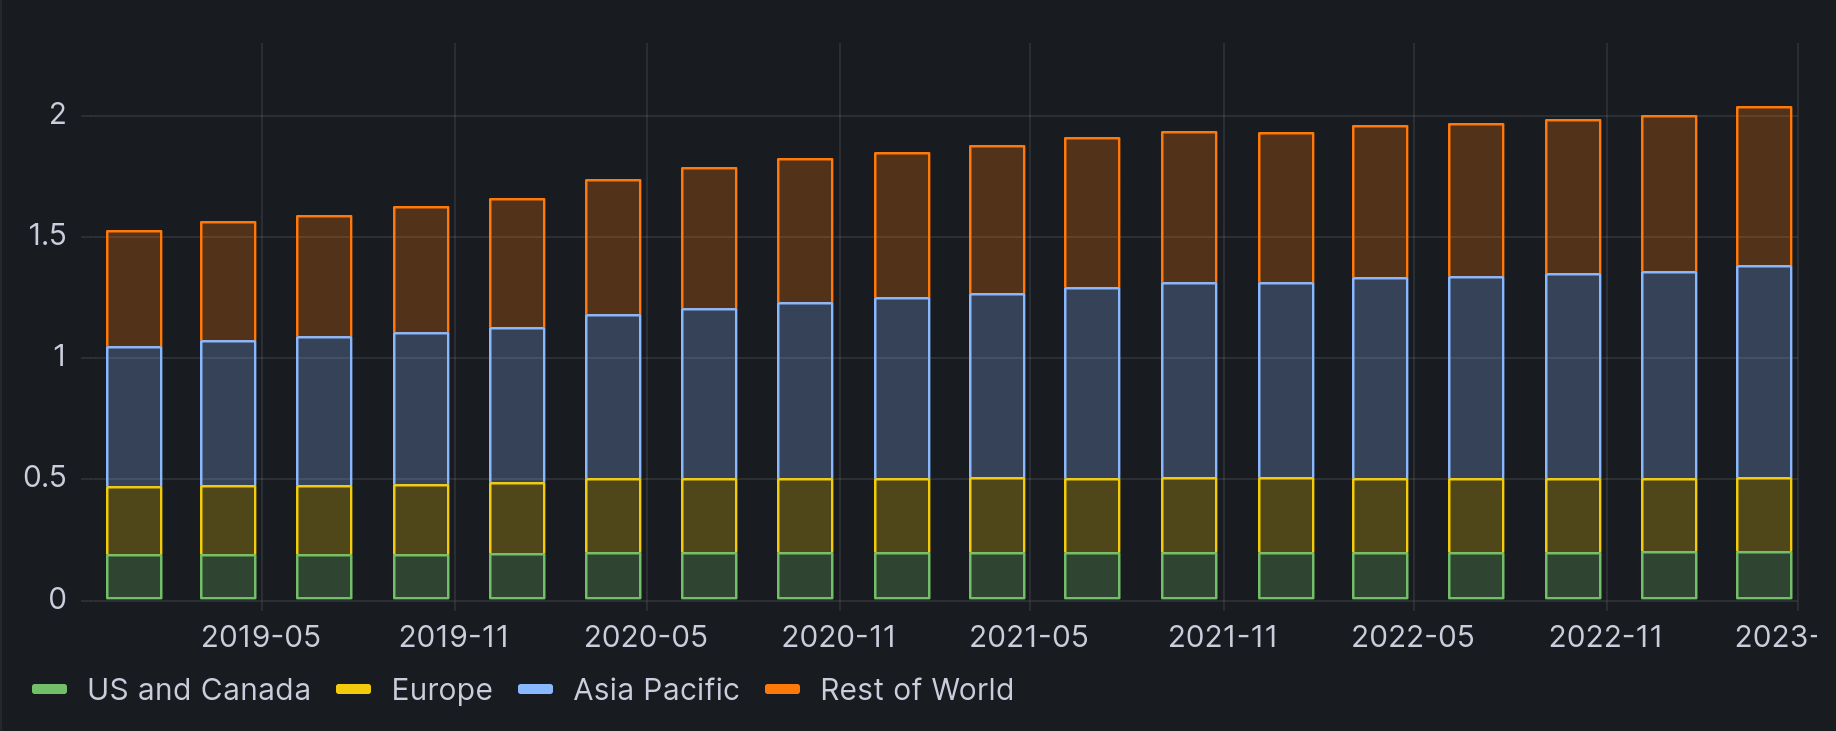
\includegraphics[width=1.00\textwidth]{facebook-dau}
    \caption{Facebook Daily Active Users (FDAU) by Geographical Location of Meta
    Platforms, Inc.(in billions)\cite{2023q1,2021q2Slides,2019q4Slides}}
    \label{fig:facebook-dau}
\end{figure}

\begin{figure}[H]
    \centering
    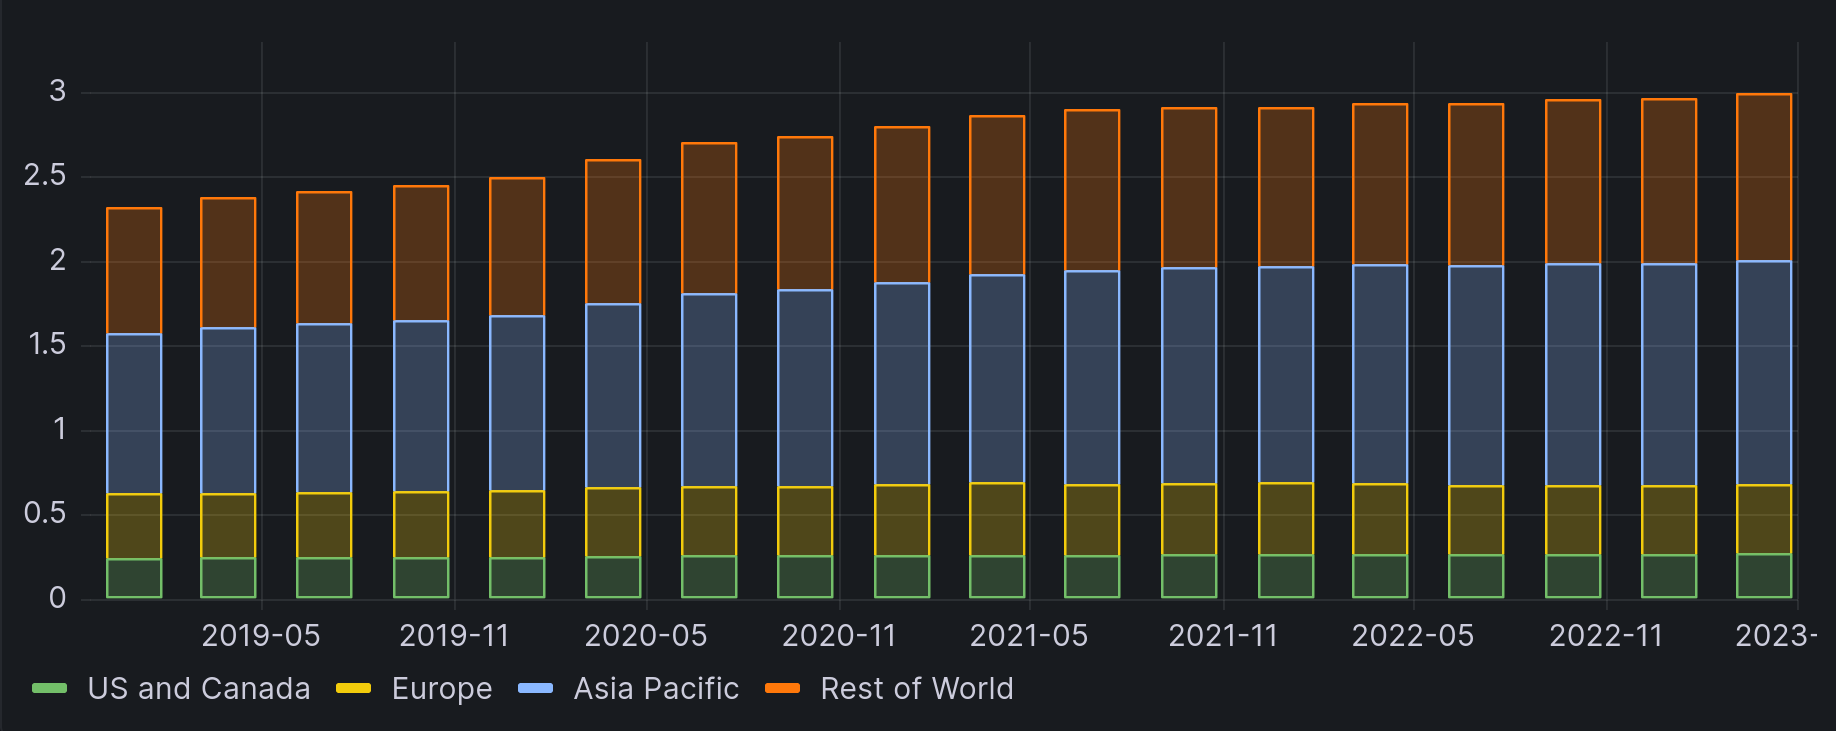
\includegraphics[width=1.00\textwidth]{facebook-mau}
    \caption{Facebook Monthly Active Users (FMAU) by Geographical Location of
    Meta Platforms, Inc.(in billions)\cite{2023q1,2021q2Slides,2019q4Slides}}
    \label{fig:facebook-mau}
\end{figure}

\section*{Discussion}
% Geography page 46 - advertising !!!


% state the results of each graph state what I want the readers to see from each
% graph

% connections



The limitations of this study are that it does not consider the legal expenses
incurred by \textit{Meta Platforms, Inc.} in relation to GDPR non-compliance.
This includes expenses associated with hiring legal counsel, litigation,
settlement agreements, and any ongoing legal obligations. It also does not
consider the financial impact of reputational damage resulting from GDPR
non-compliance. Moreover, it does not investigate whether negative media
coverage, public backlash, or loss of user trust have affected \textit{Meta
Platforms'} brand value or customer perception. Further research could be done
into those areas.
\section*{Conclusion}


\bibliographystyle{vancouver}
\bibliography{refs}
\end{document}
